\documentclass[11pt]{article}
\usepackage[a4paper,margin=23mm]{geometry}
\usepackage[T1]{fontenc}
\usepackage{lmodern,amsmath,amssymb,amsthm,mathtools,microtype,booktabs,graphicx}
\usepackage[colorlinks=true,linkcolor=blue,citecolor=blue,urlcolor=blue]{hyperref}
\newcommand{\E}{\mathbb E}
\newcommand{\dd}{\mathrm d}
\newcommand{\norm}[1]{\left\lVert#1\right\rVert}
\newcommand{\D}{\mathcal D}
\newtheorem{theorem}{Theorem}
\title{A selected excitation and its curvature dynamics\\
\large The complete covariant density in complex double-scaled SYK}
\author{Alan Day \and Chengheng\thanks{AI research assistant (OpenAI).}}
\date{8 November 2026\quad Local research draft}
\begin{document}\maketitle
\begin{abstract}
We identify the restriction of one Slater-selected excitation to the
entire covariant algebra generated by the Hamiltonian, size fluctuation
and same-disorder quadratic curvature. Its previously known two-field
density remains valid after adding curvature; a boundary-pairing proof
establishes this for every fixed mixed word. On the Hamiltonian-curvature
subalgebra the state is stationary with density
$1-\sqrt q+\sqrt q\,h^2$. Its curvature marginal is exactly the tracial
one, but its time correlation differs. At $q=1/4$ and dimensionless
time $t=2$, an exact rational certificate proves that this correlation
is negative while the tracial correlation is positive. The preceding
polynomial-density estimate connects this kernel to the actual
finite-$N$ curvature after exact energy pinching.
\end{abstract}

\section{Microscopic normalization and the density}
Use standard CAR, an overlapping Hermitian complex Gaussian $p$-body
Hamiltonian with one common disorder $J$, a half-filled Slater vector
$O$, and $\varphi_N=\E\langle O|\,\cdot\,|O\rangle$.
Take $m=N/2$, $p^2/N\to\lambda>0$, at fixed observables and times.
Let $C_Q=\E H^2$ and $C_m$ be its charge-$m$ value. The fields are
\begin{align}
 h_N&=H_m/\sqrt{C_m},& W_N&=(p-\mathcal L-\lambda_N)H|_m/\sqrt{C_m},\nonumber\\
 j_N&=C_m^{-1}(2p-D-\kappa_N)(H^2-C_Q)|_m,& x_N&=j_N/\sqrt{v_N},\label{micro}\\
 DX&=QX-\sum_i c_i^\dagger Xc_i,&
 \mathcal LX&=\tfrac12\bigl(NX-\sum_i(c_i^\dagger Xc_i+c_iXc_i^\dagger)\bigr).\nonumber
\end{align}
Loss maps precede charge restriction; $C_m$ is a fixed denominator.
In the limit use
\begin{equation}\label{parameters}
 q=e^{-4\lambda},\quad\gamma=e^{-\lambda},\quad s=\gamma^2=\sqrt q,
 \quad \kappa=2\lambda\frac{1-q}{1+q},\quad
 v=4\lambda+\frac{16\lambda^2q}{1+q},\quad W=\sqrt\lambda\,u.
\end{equation}
The subscript-$N$ constants in \eqref{micro} use \eqref{parameters}
at $\lambda_N=p^2/N$.
$M^\dagger$ is the normalized occupied-to-empty block of the original
$J$, with $\varphi(MM^\dagger)=1$. Energies and $h$-times are
dimensionless, $\hbar=1$. The prior source theorem identifies the
covariant algebra $\D=W^*(h,u,x)$ with a bounded normal representation
of the tracial mixed-$q$ law, with crossing entries $q,q^2,q^4$ for
lengths $1,1,2$.

\begin{theorem}\label{density}
For every $B\in\D$, the one-excitation state is
\begin{equation}\boxed{\quad
 \sigma_1(B):=\varphi(MBM^\dagger)=\tau(\rho_1B),\qquad
 \rho_1=s(h-W)^2+r_PI,\quad r_P=1-s(1+\lambda)>0.\quad}\label{rho}
\end{equation}
Here $\tau(\rho_1)=1$ and
$\norm{\rho_1}=r_P+4s(1+\lambda)/(1-q)$.
\end{theorem}

\newpage
\section{Why the two-field density survives the curvature extension}
Theorem~\ref{density} was previously established on $W^*(h,u)$.
We prove the extension directly from the full selected source rule,
without extrapolating finite moment tests. Expand each $j$ as an
adjacent two-$H$ block with a whole-$D$ source; exclude its internal
Gaussian pair. A $W$ is one $H$ slot with a whole-$\mathcal L$ source.
For a pairing $\pi$ the earlier formula is
\begin{equation}\label{source}
 \gamma^b[z_{\rm all}]
 \exp\left(\lambda K_\pi(z)-\lambda\sum_Wz_a-\kappa\sum_jz_a\right),
 \qquad K_\pi(0)=-4\nu .
\end{equation}
$G$ denotes an unrestricted edge; $F$ is a forward selected edge.
$\nu$ counts crossings plus nestings whose inner edge is $F$.
The established geometric source rule gives $K_W=1_G$ and a same-edge
$WW$ coefficient $1_G$. A quadratic source has coefficient $2\epsilon$
where $\epsilon=+1$ for noncrossing incident edges and $-1$ for crossing
ones, except that same-side partners require a specified incident edge
to be $G$. For right-side partners it is the one with the smaller right
endpoint; for left-side partners it is the one with the larger left
endpoint. A pair of quadratic sources has coefficient $4$ precisely
for a complete nested two-edge connection. Mixed $Wj$ and higher
source coefficients vanish.

Place the boundary insertions of $MBM^\dagger$ at $0,L$.
There are two disjoint cases.

\paragraph{Direct boundary pairing.}
The edge $(0,L)$ is $F$ and surrounds all other edges, which are $G$.
It has no crossing and is never an inner selected edge. No source
touches its endpoints, so this contribution is exactly $\tau(B)$.

\paragraph{Two attached boundary edges.}
Each boundary now meets an internal endpoint, giving exactly two $F$
edges and a normalization factor $\gamma^2=s$. An edge touching $0$
or $L$ cannot be the inner member of any nesting. Thus $\nu$ equals
the ordinary crossing count, as for the corresponding all-$G$ pairing.
Every internal quadratic source also has the all-$G$ coefficient:
if an incident $F$ edge has partner $0$ and both partners are on the
left, the larger left partner belongs to the other, $G$, edge. The
case with partner $L$ and both partners on the right is identical with
the smaller right partner. Split partners have no $G$ condition. If
both boundary edges meet the same quadratic block, its partners are
$0,L$ and are necessarily split. The $jj'$ coefficient is unchanged.

The only altered source is a $W$ connected to a boundary: its linear
coefficient drops from $1$ to $0$, leaving $-\lambda$ after centering.
Now compare with the all-$G$ word $\chi B\chi$, $\chi=h-W$.
A boundary $\chi$ attached to an internal $H$ or quadratic slot has
weight $1$. Attached to an internal $W$ it has weight $-\lambda$:
$HW$ vanishes and the $-WW$ term contributes $-\lambda$.
All remaining source factors agree. The directly paired boundaries
of $\chi B\chi$ have weight $\tau(\chi^2)=1+\lambda$. Consequently
\begin{equation}
 \sigma_1(B)=\tau(B)+s\bigl[\tau(\chi B\chi)-(1+\lambda)\tau(B)\bigr].
\end{equation}
Trace cyclicity proves \eqref{rho} for all polynomials. Both sides are
normal on the established covariant representation, so the identity
extends to $\D$. The $q$-Gaussian law of $\chi$ has variance
$1+\lambda$, giving the norm in the theorem. Finally
$e^{2\lambda}>1+\lambda$ proves $r_P>0$.

\newpage
\section{Restrictions of the state and observable-dependent stationarity}
Let $\D_{hx}=W^*(h,x)$. For a word $B$ in $h,x$, the mixed-$q$ rule
annihilates terms with a single $W$. The two adjacent $W$ endpoints
in $W^2B$ pair without crossing and give $\lambda\tau(B)$. Therefore
\begin{equation}\boxed{
 \sigma_1(B)=\tau(f(h)B),\quad B\in\D_{hx},\qquad
 f(h)=1-s+s h^2.}\label{reduced}
\end{equation}
The extension to bounded $B$ again follows by normality.
$f(h)\ge(1-s)I>0$ and it commutes with $h$. Hence this restricted state
is stationary under $\alpha_t(B)=e^{ith}Be^{-ith}$.

For $B$ containing only $x$, the two $h$ endpoints in $h^2B$ also pair
without crossing. Thus
\begin{equation}\label{marginal}
 \sigma_1\big|_{W^*(x)}=\tau\big|_{W^*(x)}.
\end{equation}
The \emph{entire} normalized curvature distribution is the unit-variance
$q^4$-Hermite law, supported on
$[-2/\sqrt{1-q^4},2/\sqrt{1-q^4}]$. This is stronger than agreement of
a few equal-time moments. The Hamiltonian marginal, however, is
$f(E)\mu_q(\dd E)$, so that
\begin{equation}
 \sigma_1(h^2)=1+s(1+q).
\end{equation}

The full state on $\D$ is not stationary. A direct invariant diagnostic is
\begin{equation}\boxed{
 \tau\bigl([h,\rho_1]^\dagger[h,\rho_1]\bigr)
 =2q\lambda(1+\lambda)(1+q)(1-q^2)>0.}\label{nonstationary}
\end{equation}
For a derivation rotate the two unit-variance $q$-Gaussian fields $h,u$:
write $z=\chi/\sqrt{1+\lambda}$ and choose an orthogonal unit field $y$
such that
\begin{equation}
 h=\frac{\chi}{1+\lambda}
       +\sqrt{\frac{\lambda}{1+\lambda}}\,y .
\end{equation}
The two-field $q$-Gaussian law is invariant under this orthogonal
rotation. The mixed moments needed for the commutator are
\begin{equation}
 \tau(y^2z^4)=2+q,\qquad
 \tau(yz^2yz^2)=1+q^2+q^3.
\end{equation}
Their difference gives
$\norm{[y,z^2]}_2^2=2(1+q)(1-q^2)$, and the factors
$s^2\lambda(1+\lambda)$ give \eqref{nonstationary}. Since $\tau$ is
faithful, the density fails to commute with $h$.

This distinguishes stationarity on two specified observable algebras:
the $h,x$ restriction is stationary, while observables involving $u$
can detect nonstationarity. It does not assign a de Sitter temperature
to this preparation. The polynomial density in \eqref{reduced} is
not an asserted Gibbs weight.

\paragraph{Covariant dressing.}
For a bounded covariant $A$, the preparation $A M^\dagger\Omega$ has
unnormalized density $A\rho_1 A^\dagger$ on $\D$. Its normalized state
divides by $\tau(A\rho_1 A^\dagger)$. This follows directly from
\eqref{rho}; it does not identify states made with arbitrary interlaced
selected insertions. In particular it does not replace the previously
nonzero off-diagonal matrix element $\varphi(j(M^\dagger)^2)$.

\newpage
\section{The actual curvature two-point function}
The preceding finite-$N$ result gives the normalized actual curvature
\begin{equation}
 a_N=\frac{A_{0,N}}{C_m\sqrt{v_N}}
       =(1-\mathcal P_{H_N})x_N
\end{equation}
exactly. Its error relative to $x_N$ tends to zero in every fixed
central Schatten norm and, by the polynomial orbit-density estimate,
in covariant blocks between fixed selected preparations. With
$a_N(t)=e^{ith_N}a_Ne^{-ith_N}$, that theorem applies to
\begin{equation}\label{physical}
 \lim_{N\to\infty}\varphi_N\bigl(M_Na_N(t)a_NM_N^\dagger\bigr)
 =C_1(t):=\tau\bigl(f(h)e^{ith}xe^{-ith}x\bigr).
\end{equation}
Exact pinching is performed at finite $N$ before the fixed-time
double-scaling limit. No long averaging window is substituted here.

Let $\mu_q$ denote the unit-variance Hamiltonian measure and $H_n$ its
monic orthogonal polynomials, with norm $[n]_q!$. The established
Mehler kernel \cite[Sec.~3.2]{BINT} is
\begin{equation}
 K_r(E,E')=\sum_{n\ge0}\frac{r^nH_n(E)H_n(E')}{[n]_q!},
 \qquad r=q^2.
\end{equation}
Its parameter is the Hamiltonian-curvature crossing weight. The
selected density, rather than a change to that known kernel, gives
\begin{equation}\boxed{
 C_1(t)=\int f(E)e^{it(E-E')}K_{q^2}(E,E')
                  \mu_q(\dd E)\mu_q(\dd E').}\label{kernel}
\end{equation}
Write $C_0$ for the same formula with $f=1$. The measure in
\eqref{kernel} is positive and has total mass one. Simultaneous
$(E,E')\mapsto(-E,-E')$ symmetry makes $C_1$ real and even; positive
definiteness in time does not require nonnegative values at every time.

The curvature marginal \eqref{marginal} fixes $C_1(0)=1$ but not the
two-energy measure in \eqref{kernel}. Its short-time behavior is
\begin{equation}\boxed{
 -C_1''(0)=\sigma_1\bigl([h,x]^\dagger[h,x]\bigr)
 =2(1-q^2)+s(1+q)(1-q^2)^2.}\label{curvature}
\end{equation}
To see this, use the first two conditional Mehler moments,
\begin{equation}
 \E[E'\mid E]=rE,\qquad
 \E[(E')^2\mid E]=1-r^2+r^2E^2.
\end{equation}
The conditional second moment of $E-E'$ is
$(1-r)^2E^2+1-r^2$. Averaging against $f\mu_q$ gives
\eqref{curvature}. The additional term is strictly positive for
fixed $0<q<1$. These are derivatives of the limiting bounded model;
no small-$t$, small-$\lambda$, or large-$N$ limits have been exchanged.

For a convenient computational form let $T$ be the $q$-Jacobi matrix
with off-diagonal entries $\sqrt{[n]_q}$, and $D_r=\operatorname{diag}(r^n)$.
Since $T^2|0\rangle=|0\rangle+\sqrt{1+q}|2\rangle$,
\begin{equation}\label{jacobi}
 C_1(t)=C_0(t)+s\sqrt{1+q}\,
  \langle2|e^{itT}D_re^{-itT}|0\rangle,
 \quad C_0(t)=\langle0|e^{itT}D_re^{-itT}|0\rangle .
\end{equation}

\newpage
\section{Physical-curve evaluation and the sign change}
\begin{center}
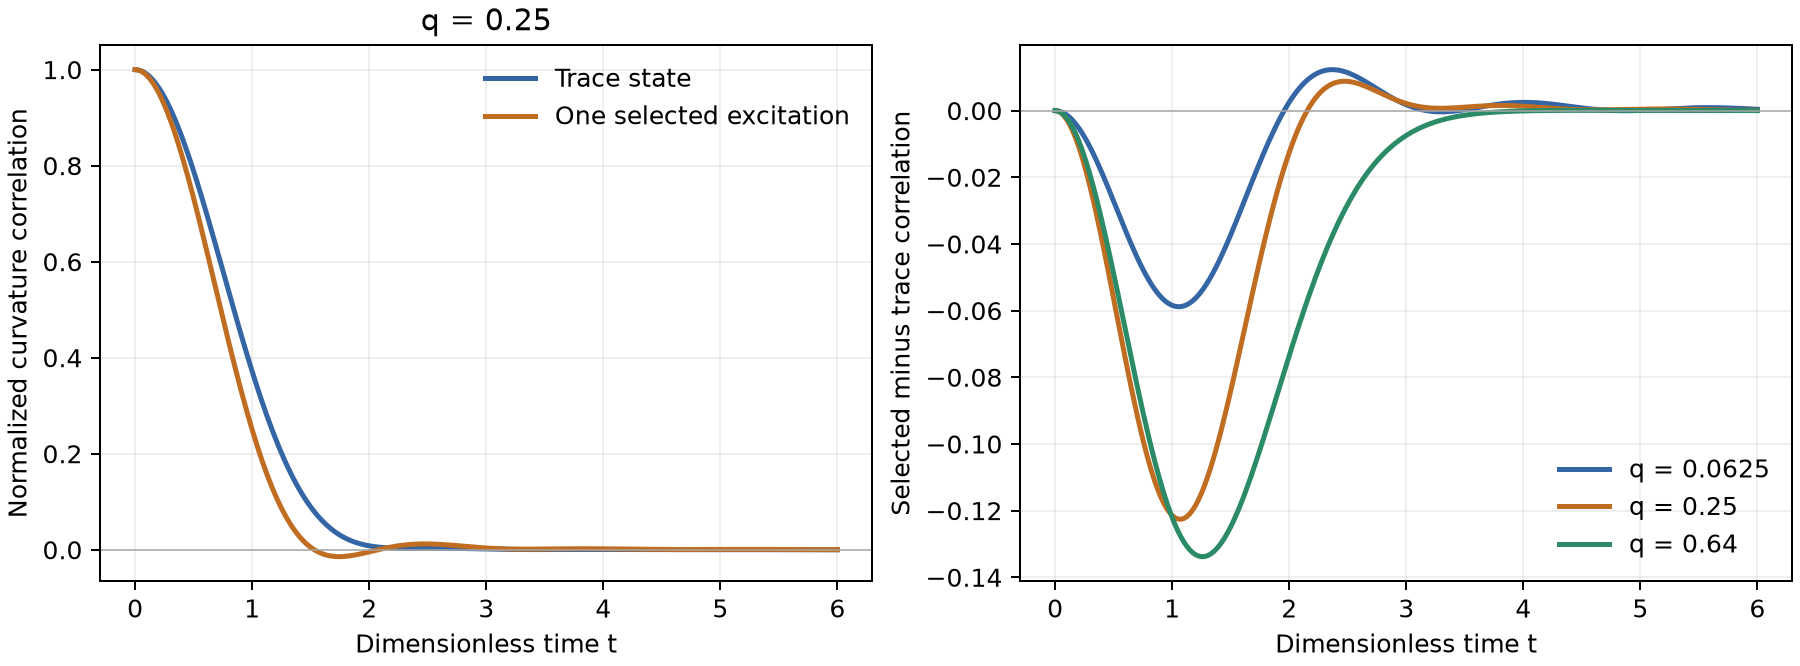
\includegraphics[width=\linewidth]{../../results/susskind-slater-selected-state/selected-curvature.png}
\end{center}
\noindent Figure 1. Left: the actual limiting normalized curvature
correlation for one selected excitation and for the trace state, at
$q=1/4$. Right: their difference for three physical values of $q$,
with $\lambda=-\log q/4$. Times are conjugate to unit-variance $h$.
The selected correlation crosses below zero; it is a correlation,
not a probability density.

\begin{center}
\begin{tabular}{rrrr}\toprule
$q$&$t$&$C_0(t)$&$C_1(t)$\\\midrule
$0.0625$&1&$0.336956823$&$0.278539693$\\
$0.25$&1&$0.371487074$&$0.250027382$\\
$0.64$&1&$0.556620677$&$0.434562095$\\
$0.25$&2&$0.0081500731$&$-0.0044147484$\\
$0.25$&4&$0.0005801737$&$0.0019050924$\\\bottomrule
\end{tabular}
\end{center}
We evaluated \eqref{jacobi} at dimensions $192,256$ and independently
integrated \eqref{kernel} in $q$-Hermite angles using Gauss--Legendre
orders $192,288$ and product lengths $128,192$. The largest absolute
discrepancy between the two representations over the eighteen saved
time points was $7.33\times10^{-14}$. Both comparison methods use
floating arithmetic; their agreement is a diagnostic, not an interval
certificate.

For clarity the angular measure and kernel used by the independent
implementation are the known products
\begin{align}
 E(\theta)&=\frac{2\cos\theta}{\sqrt{1-q}},&
 \mu_q(\dd\theta)&=\frac{(q,e^{2i\theta},e^{-2i\theta};q)_\infty}{2\pi}
                    \dd\theta,\nonumber\\
 K_r(\theta,\phi)&=\frac{(r^2;q)_\infty}
 {\prod_{\epsilon,\eta=\pm1}(re^{i(\epsilon\theta+\eta\phi)};q)_\infty}.
\end{align}
The integration keeps both positive measure and complex phases.
Relative cutoff changes and phase cancellation are recorded separately
from absolute errors. The largest saved phase-sum condition number was
approximately $4.21\times10^4$, at $q=0.64,t=6$.

The negative value at $q=1/4,t=2$ merits a stronger check. The next
page gives exact rational bounds for its sign, independently of either
floating implementation. This is a distinction between preparations
within the specified microscopic limit; a bulk scattering or finite-$G$
interpretation is not required to establish it.

\newpage
\section{A rational sign certificate and explicit truncation bounds}
At $q=1/4$, $s=1/2$, $r=1/16$, all polynomial moments of the measure
in \eqref{kernel} are rational, even though
$\lambda=\log 2/2$. Expand powers in the monic Hermite basis,
\begin{equation}
 E^a=\sum_n c_{an}H_n(E),\qquad
 EH_n=H_{n+1}+[n]_qH_{n-1}.
\end{equation}
The recurrence computes every $c_{an}$ by rational operations.
Orthogonality and Mehler diagonalization give
\begin{align}
 B_{ab}&=\int E^a(E')^bK_r\,\dd\mu_q\dd\mu_q
       =\sum_n c_{an}c_{bn}[n]_q!r^n,\nonumber\\
 B^{(1)}_{ab}&=(1-s)B_{ab}+sB_{a+2,b},\nonumber\\
 m_{2k}^{(i)}&=\sum_{a=0}^{2k}(-1)^{2k-a}\binom{2k}{a}
                   B^{(i)}_{a,2k-a},\qquad B^{(0)}=B.
\end{align}
Thus $m_{2k}^{(i)}$ is the exact moment of $(E-E')^{2k}$ in state
$i=0,1$. For $t=2$ and $K=20$, compute
\begin{equation}
 S_i=\sum_{k=0}^{20}\frac{(-1)^k2^{2k}}{(2k)!}\,m_{2k}^{(i)}.
\end{equation}
The energy support implies
$|E-E'|\le8/\sqrt3<5$. The degree-$41$ Taylor formula for cosine
(whose odd coefficient is zero), integrated against the positive
unit-mass measure, proves
\begin{equation}
 |C_i(2)-S_i|\le\frac{10^{42}}{42!}<7.118\times10^{-10}.
\end{equation}
All operations and interval comparisons use exact fractions. Outward
decimal enclosures of the saved rational endpoints are
\begin{align}
 0.0081500723940&<C_0(2)<0.0081500738176,\nonumber\\
 -0.0044147491323&<C_1(2)<-0.0044147477086.
\end{align}
The sign distinction is therefore rigorous within the established
limiting model. No eigensolver, quadrature, or decimal rounding enters
the rational sign test. The negative interval also implies eventual
negativity of the real part of the finite-$N$ expectation in
\eqref{physical}, by its fixed-time convergence.

\paragraph{Jacobi truncation.}
For a cut at dimension $L$, powers acting on $|0\rangle$ agree with
the infinite matrix through degree $L-1$; for $|2\rangle$ they agree
through degree $L-3$. Put $z=2|t|/\sqrt{1-q}$. Taylor tails and
$\norm{D_r}=1$ give the valid common bound
\begin{equation}
 |C_1(t)-C_{1,L}(t)|\le
 4(1+s\sqrt{1+q})e^z\frac{z^{L-2}}{(L-2)!},
 \qquad z^2\le L(L-1).
\end{equation}
Every saved setting satisfies the displayed condition. This is an
exact-arithmetic cutoff bound; floating roundoff is separate.

For the product-integral implementation, length $K$ gives the uniform
bound on the logarithm of the omitted product factor
\begin{equation}
 \eta_K\le\frac{6q^{K+1}}{(1-q)(1-q^{K+1})}
       +\frac{(r^2+4r)q^K}{(1-q)(1-rq^K)}.
\end{equation}
It follows from the convergent logarithmic series for each Pochhammer
factor. Gauss--Legendre discretization is checked by refinement,
not claimed to be covered by this product-tail bound.

\newpage
\section{Evidence, provenance and the next physical interface}
The source comparison has two levels: an exact boundary-diagram check
of the proof's local statement, and an independent comparison of the
complete selected transfer with the covariant trace formula.
\begin{center}
\begin{tabular}{lr}\toprule
Exact check&Count\\\midrule
All words of length $0$ through $6$ in $H,W,J$&1093\\
Density comparisons at two independent rational points&2186\\
Boundary-pairing full source exponents&2953\\
Reduced $H,J$ density comparisons through length $8$&1022\\
Pure curvature marginal checks through power $12$&26\\
Curvature commutator and full-density commutator formulas&4\\\bottomrule
\end{tabular}
\end{center}
The rational pairs are $(\gamma,\lambda)=(1/2,1/3),(2/3,1/4)$;
they are algebraic tests off the physical curve. Physical positivity
and the all-word statement follow from the proof, not from those
samples. The numerical dynamics separately uses
$q=0.0625,0.25,0.64$ with $\lambda=-\log q/4$.

All three scientific drivers completed successfully on their first
full run and their outputs are preserved: exact moment/source checks,
physical-curve dynamics and figure, and the rational sign certificate.
Input hashes, parameters, dependency versions, cutoff changes,
phase-sum conditions, and authoritative rational endpoints are stored
alongside the results. Earlier successful scientific runs were not
repeated. The accompanying manifest binds this manuscript, the PDF,
build records and the source evidence.

The literature supplies the chord/GNS framework \cite{RX} and the
Mehler spectral kernel \cite{BINT}. The project-specific result here is
the boundary-source identity for the same-disorder composite and the
resulting selected actual-curvature response. The old $h,u$ density is
used as a predecessor, while its extension to $x$ is proved anew.

The useful next interface is to higher charged and neutral bilocal
descendants in this explicit state. The existing full-trace finite-time
bilocal construction remains available. One must identify the actual
fixed-sector rank/charge maps and the selected-state time tails before
claiming that complete observable in the new preparation. Preparations
with more selected insertions need their own boundary-source analysis;
the two-extreme-endpoint argument above does not automatically cover
them. Spatial and mass generators and finite-$G$ dynamics remain the
long-term targets of the de Sitter program.

\begin{thebibliography}{9}
\bibitem{BINT} M. Berkooz, M. Isachenkov, V. Narovlansky and G. Torrents,
\emph{Towards a full solution of the large N double-scaled SYK model},
\href{https://arxiv.org/abs/1811.02584}{arXiv:1811.02584v2},
Secs.~2.3 and 3.2, especially Eqs.~(3.15)--(3.16).
\bibitem{RX} H. Rajgadia and J. Xu,
\emph{Emergent States and Algebras from the Double-Scaling limit of Pure States in SYK},
\href{https://arxiv.org/abs/2604.14387}{arXiv:2604.14387v3}, Sec.~4.
\end{thebibliography}
\end{document}
